% 
%% SOSP 2017 Template
%%
%% Uses sigplanconf from:
%% 
%%    http://www.sigplan.org/sites/default/files/sigplanconf.cls
%%
%% with 10pt and preprint options. 
%%
%% Replace 'XX' with your paper number (assigned when you register abstract)
%% Replace 'NN' with actual number of pages. 

\documentclass[10pt]{sigplanconf}
\usepackage{times}

\usepackage{datetime}
\usepackage{url}
\usepackage{hyperref}
\usepackage{graphicx}
\usepackage{listings}
\copyrightyear{2017} 


% These only appear when the 'preprint' option is specified.
% Enabling these will cause the first page of the document to fail the 
% format check on HotCRP :-(
%\titlebanner{Under submission to SOSP 2017 - do not cite or distribute}
%\preprintfooter{Draft of {\currenttime}, \today{}}

% No date in title area.
\date{}

% Paper number and no. of pages as author
\authorinfo{Keyan Chen(kc32),  Zhiyuan Tang(zt6)}{7 pages}


% Actual document begins below.
\begin{document}

\title{Generic Mutex Subsystem of Linux Kernel} 
\maketitle

\begin{abstract}

\begin{itemize}
	\item Motivation: Both of us are computer science undergraduate students and we are all very interested in parallel programming. While we were taking COMP322 last year, we found out, astonishingly, that the choice of different locking mechanisms such as mutex, shared-locks, exclusive-locks, and semaphores can have a significant influence on the overall performance of the program. Therefore, in order to have a better understanding of multi-thread programming and gain more knowledge into the locking mechanisms that we used before, we decided to research on mutex subsystem of linux kernel.
	\item Problem Statements: Our main goal of the research is to understand the implementation details and design highlights of linux kernel mutex subsystem, as well as its advantages over other locking mechanisms and its predecessors. Lastly, as suggested by Dr. Zhong, we also researched on linux implementation of atomic operations. 
	\item Conclusion: In short, we should use mutex whenever possible instead of semaphore because of the various advantages of mutex over semaphore. In addition, the idea of optimistic spinning and the design of MCS lock also gave us inspirations on a lot of possible optimization that we can implement in the future in our multi-thread programs. More detailed conclusions can be found in our Conclusion section.
		
\end{itemize}

\end{abstract}


\vspace{80pt}

\section{Brief History and Background}

In the linux kernel, mutex refers to a particular locking primitive that enforces serialization on shared memory systems in order to protect critical sections from undesired concurrent data access. \\
Before 2006, when developers wanted to gain mutual exclusion among their shared memory systems, they would use binary semaphores, which are sleeping locks. However, Mutexes were introduced in 2006 as an alternative to binary semaphores and this new data structure provided a number of advantages, including simpler interfaces, and at that time less amount of code. 

\subsection{Why Mutex?}
Why do we need a new mutex subsystem? And what are the problems with semaphores?\\
\begin{enumerate}
	\item 'struct mutex' takes less space.
	\begin{enumerate}
		\item On x86, 'struct semaphore' is 20 bytes, while 'struct mutex' is 16 bytes. A smaller structure size means less RAM footprint, and better CPU-cache utilization
	\end{enumerate}
	\item Mutex can result in tighter code
	\begin{enumerate}
		\item On x86 we can get the following .text sizes when switching all mutex-alike semaphores in the kernel to the mutex subsystem
		\begin{figure}[h!]
			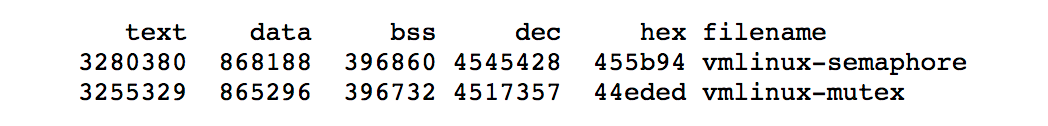
\includegraphics[scale=0.5]{image00.png}
		\end{figure}
		\item That's 25021 bytes of code saved, or a 0.76\% win off the hottest codes paths of the kernel
		\item Less code means better in-cache footprint, which is one of the major optimization goals in the linux kernel when people were proposing the addition of mutex subsystem in 2006. 
	\end{enumerate}
	\item The mutex subsystem is faster and has superior scalability for contented workloads.
	\begin{enumerate}
		\item On a 8-way x86 system, running a mutex based kernel and testing create+unlink+close(of separate, per-task files) in /tmp with 16 parallel tasks, the average number of ops/sec is given as follows:
		\begin{figure}[h!]
			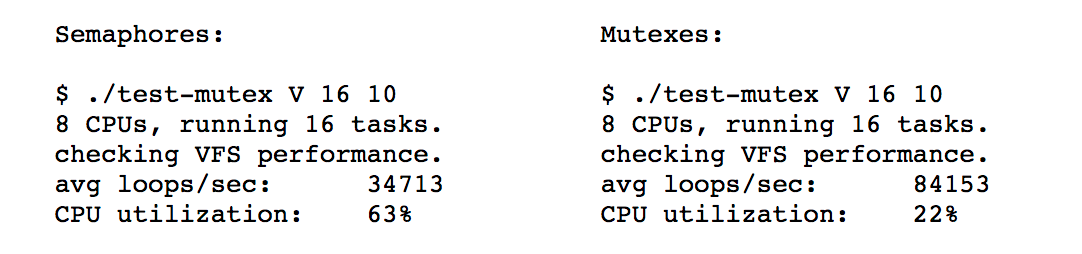
\includegraphics[scale=0.5]{image01.png}
		\end{figure}
		\item In this workload, mutex based kernel was \textbf{2.4 times} faster than the semaphore based kernel, and it also had \textbf{2.8 times} less CPU utilization. 
	\end{enumerate}
\end{enumerate}


\subsection{Design and Implementation details}
Mutex is represented by ‘struct mutex’, defined in include/linux/mutex.h and implemented in kernel/locking/mutex.c. The mutex uses a three state atomic counter to represent the different possible transitions that can occur during the lifetime of a mutex:
\begin{itemize}
	\item 1: unlocked
	\item 0: locked, no waiters
	\item negative: locked, with potential waiters
\end{itemize}
In its most basic form it also includes a wait-queue and a spinlock that serializes access to it. When acquring a mutex, there are three possible paths that can be taken, depending on the state of lock:
\begin{enumerate}
	\item Fastpath: This is the first path that mutex subsystem will take in its locking routine. It tries to atomically acquire the lock by decrementing the counter. If it was already taken by another task it goes to the next possible path. This logic is architecture specific.
	\item Mid-path: This is also known as optimistic spinning. It tries to spin for acquisition while the lock owner is running and there are no other tasks ready to run that have higher priority. The reason to have this unique optimistic spinning routine is that if the lock owner is running, it is likely to release the lock soon. Therefore, we can get significant performance boosting using this optimistic spinning routine. The mutex spinners are queued up using MCS lock so that only one spinner can compete for the mutex (more details will be discussed in section 2.2). 
	\item Slowpath: This is the last step to take if the above two steps all fail. If the lock is still unable to be acquired, the task is added to the wait-queue and sleeps until woken up by the unlock path. Under normal circumstances it blocks as TASK\_UNINTERRUPTIBLE.
\end{enumerate}

\vspace{50pt}

\section{Interesting Findings}
\subsection{Unique Optimistic Spinning in Linux Mutex Subsystem}
While formally kernel mutexes are sleepable locks, it is the Mid-path(aka optimistic spinning) that makes the mutex subsystem now more practically a hybrid type. By simply not interrupting a task and busy-waiting for a few cycles instead of immediately sleeping, the performance of this lock has been seen to significantly improve a number of workloads. \\

\begin{figure}[h!]
	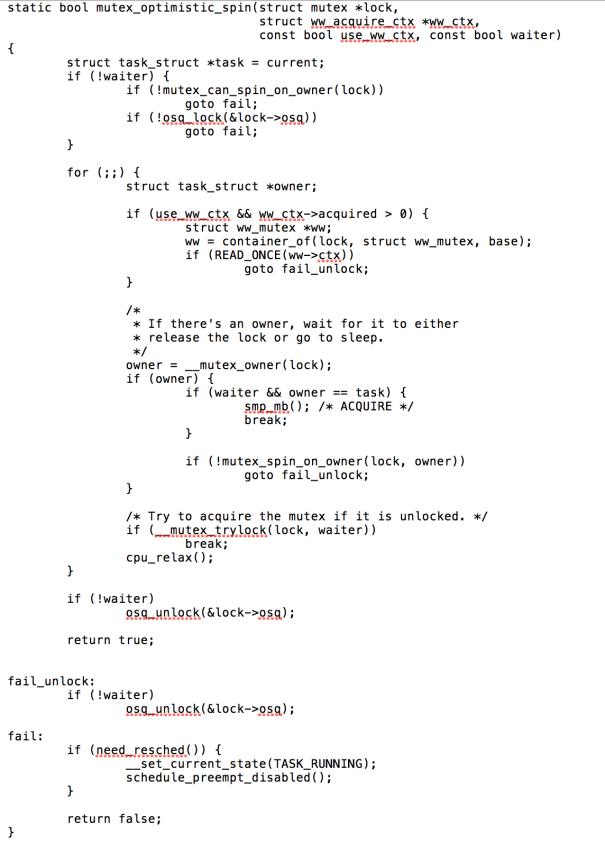
\includegraphics[scale=1]{image02.png}
	\caption{Optimistic Spinning routine in the source code}
\end{figure}

\vspace{50pt}
\subsection{Design and Use of MCS locks in linux kernel}
In mutex subsystem, mutex spinners are queued up using MCS locks as described about above. 
The design of MCS lock and the difference between MCS lock and ordinary spinlock is also a very interesting design decision in linux kernel.\\
The concept of a spinlock is simple and straight-forward. When a thread wants to acquire the lock it will attempt to set the lock bit of that spinlock with an atomic compare-and-swap(CAS) instruction and repeatedly spin there if the lock can not be acquired during one CAS. \\
However, spinlocks have some fundamental problems. The biggest problem is the cache-line bouncing results from the fact that every attempt to acquire the lock requires moving the cache containing the lock to local CPU. This cache-line bouncing can have detrimental effect on the performance of contended locks. Therefore, developers have been working on reducing the cache contention of spinlocks and as a result, MCS locks were introduced by Tim Chen to solve this problem.\\
The structure of MCS lock is defined in struct mcs\_spinlock\\
\begin{figure}[h!]
	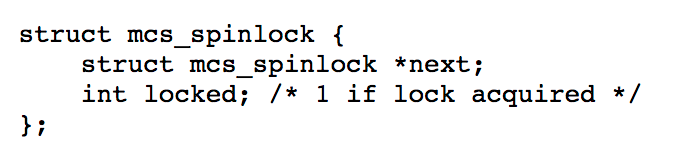
\includegraphics[scale=0.7]{mcslock0.png}
\end{figure}\\
Here we will go step-by-step to demonstrate how a MCS lock works and thus, we can see the difference between MCS lock and ordinary spinlock, as well as why MCS lock is guaranteed to provide a FIFO ordering on unlocking waiting threads. \\

\begin{itemize}
	\item From the declaration of struct mcs\_spinlock we can visualize an unlocked MCS lock as the following. Note that the next pointer is currently a null pointer because nobody has owned this mcs\_spinlock yet. 
	\begin{figure}[h]
		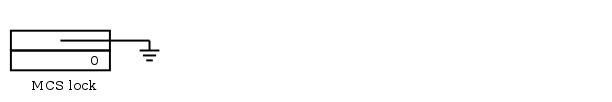
\includegraphics[scale=0.4]{mcslock1.png}
	\end{figure}\\
	\item Now when a new CPU thread is going to acquire the MCS lock, it will instantiate a mcs\_spinlock structure on its own thread and use an atomic exchange operation to try to store the address of its own mcs\_spinlock in the next field of the main MCS lock. The atomic exchange will return the previous value of the main MCS lock's next field. In this case when the previous next value of null pointer is returned back to the CPU thread acquiring the lock, the CPU thread will know that it successfully acquires the lock because nobody has already set the next pointer of main MCS lock. At this point the system can be visualized in this figure:\\
	\begin{figure}[h!]
		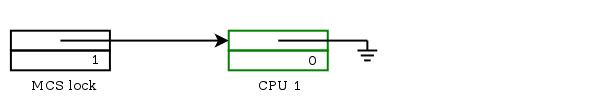
\includegraphics[scale=0.4]{mcslock2.png}
	\end{figure}\\
	\item The most interesting thing comes to our view when a second CPU thread is going to acquire the same MCS lock. If there's a second CPU thread trying to acquire the MCS lock while the lock hasn't been unlocked yet, the thread will still try the same locking routine as specified above. And then the returned mcs\_spinlock address from the atomic swap will be a pointer to the first CPU thread's mcs\_spinlock structure. In this case the second CPU will know that it hasn't acquired the MCS lock and will thus, store a pointer to its own mcs\_spinlock structure in the next field of the first CPU thread's mcs\_spinlock structure in order to form a FIFO queue. The system at this point can be visualized in this figure:
	\begin{figure}[h!]
		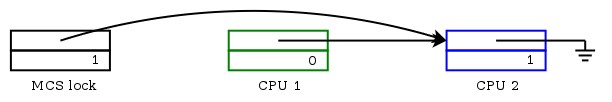
\includegraphics[scale=0.33]{mcslock4.png}
	\end{figure}\\
	\item Once this assignment is done, the second CPU thread will spin on the locked value in its own mcs\_spinlock structure rather than in the main MCS lock's structure. Therefore, the second CPU thread's spinning will be entirely CPU-local (and this is why MCS lock is a self spinning lock). As more CPU threads are joining this FIFO queue, each thread will be spinning on the locked value of its local mcs\_spinlock structure and form a chain of waiting queue, which by its structure, guarantees a FIFO unlock ordering. 
	\item Finally when the first CPU thread is going to unlock the MCS lock, it will first try to do a compare-and-swap(CAS) operation on the main MCS lock's next field to set it to null pointer. However, if it finds that the next field of the main MCS lock no longer points to itself, the CAS operation will fail. If that CAS operation fails, the first thread will know that there are other waiting threads and will thus find the mcs\_spinlock structure of the second thread and change its locked value in order to stop second thread from spinning and unlock it. The system at this point can be visualized in this figure:
	\begin{figure}[h!]
		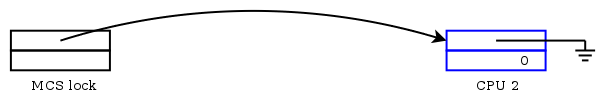
\includegraphics[scale=0.3]{mcslock5.png}
	\end{figure}
	
\vspace{30pt}
	
In conclusion, an MCS lock is more complicated than a ordinary spinlock. But the added complexity removes much of the cache-line bouncing in ordinary spinlock and ensures a FIFO unlock ordering which will save us from starvation. Therefore, mutex subsystem in linux kernel chooses to use MCS locks to queue up mutex spinners. 
\end{itemize}

\vspace{50pt}
\subsection{Bug in an obviously correct reference count code pattern}
This bug comes from a kernel crash reported in July 2013. And this bug report had not been resolved until December 2013. Because of this incident, people found out surprisingly that an "obviously correct" reference count code pattern can turn out to have potential data race problems that can lead to dangerous bugs. However, understanding this bug requires a deep understanding about linux kernel mutex subsystem, especially its unique optimistic spinning phase. Before going deep into the analysis of the bug, let's first see a piece of code, which manipulates a structure called "s" and this structure is protected by a mutex embedded with it. 
\lstset{language=C}
\begin{lstlisting}
int free = 0;

mutex_lock(&s->lock);
if (--s->refcount == 0) {
	free = 1;
}

mutex_unlock(&s->lock);
if (free) {
	kfree(s);
}

\end{lstlisting}
\vspace{10pt}
From a first look, this piece of code just "works". It simply locks s, decrements reference counter to s, detects whether we can free s, and then unlock s. However, because of the fact that current implementation of mutex has an optimistic spinning phase while acquiring the lock, this piece of code is no longer data race free. \\
The structure mutex has an atomic counter and a spinlock. When the lock is free and one thread is going to acquire lock, it will atomically decrement the counter to 0 and continue, which is known as the fast path as specified in section 1.2.\\
When the thread is going to unlock mutex, it will atomically increment counter to 1 if counter is 0, which means that there are no waiting threads on this mutex currently. If the current value of counter is negative, the mutex\_unlock() routine need to wake up the first waiting thread on mutex. In code the lifecycle of a mutex can be shown as below.
\vspace{10pt}

\begin{lstlisting}
spin_lock(&lock->wait_lock);
atomic_set(&lock->count, 1);
// wake up first waiting thread
wake_up_process(); 
spin_unlock(&lock->wait_lock);
\end{lstlisting}
\vspace{10pt}

\noindent At this point the bug gradually becomes clear to us. If currently the mutex is owned by one thread and there are other threads executing the slow path of the lock routine, which are been put into wait queue. Then there's a new thread coming in trying to acquire the lock. Because of the optimistic spinning phase, if the old mutex owner starts to release the lock when the new coming thread is currently doing optimistic spinning, then the new coming thread will immediately take the lock once it sees the effect of 
\vspace{10pt}
\begin{lstlisting}
atomic_set(&lock->count, 1);
\end{lstlisting}
\vspace{10pt}

\noindent In addition, as the original owner of the lock sees that there are threads in waiting queue, it will call
\vspace{10pt}
\begin{lstlisting}
wake_up_process(); 
\end{lstlisting}
\vspace{10pt}

\noindent to wake up the next waiting thread. \\
\noindent However, the new coming thread already enters the critical section at this point and if this new coming thread quickly frees the data structure containing the lock, the final 
\vspace{10pt}
\begin{lstlisting}
spin_unlock(&lock->wait_lock);
\end{lstlisting}
\vspace{10pt}

\noindent operation executed by the old lock owner will be applied to already freed memory space, and thus causing all sorts of problems. \\
Therefore, Linus Torvalds, the people who detected this concurrency bug, concludes:\\

\textit{In other words, it's unsafe to protect reference counts inside objects with anything but spinlocks and/or atomic refcounts. Or you have to have the lock "outside" the object you're protecting(which is often what you want for other reasons anyway, notably lookup)}\\

\vspace{50pt}

\section{Linux Implementation of Atomic Operations}
\subsection{Why we include implementation of atomic operations as part of our research on mutex subsystem}
"Only knowing how to use computer instructions without knowing how those instructions are implemented under the hood" is a pretty common description for superficial computer science students from others especially Electrical Engineering people. During our initial research into mutex subsystem, we made the same mistake of becoming such superficial computer science students. \\
Fortunately, thanks for the timely suggestion from Dr. Zhong during our project presentation, we quickly found out that our research about mutex subsystem was too constrained on a software level without going deep into the implementations of locks and atomic operations on a hardware level. Therefore, we spent a large amount of time in the later parts of our research journey on understanding the actual implementation of atomic operations.

\subsection{Intro}
Linux provides an abstraction of atomic operations. However, the implementation details vary from different architectures.\\
As what we have discussed in the final presentation, all atomic operations can be performed by disabling interrupts, emulating atomic operations, and re-enabling interrupts. The advantage of this approach is that the logic is simple and the operating system does not need special instructions from the hardware. Thus, this approach is indeed used as the most generic implementation of atomic operations. The details can be found in Linux/include/asm-generic/atomic.h and the code is posted below.\\
\begin{figure}[h!]
  \centering
  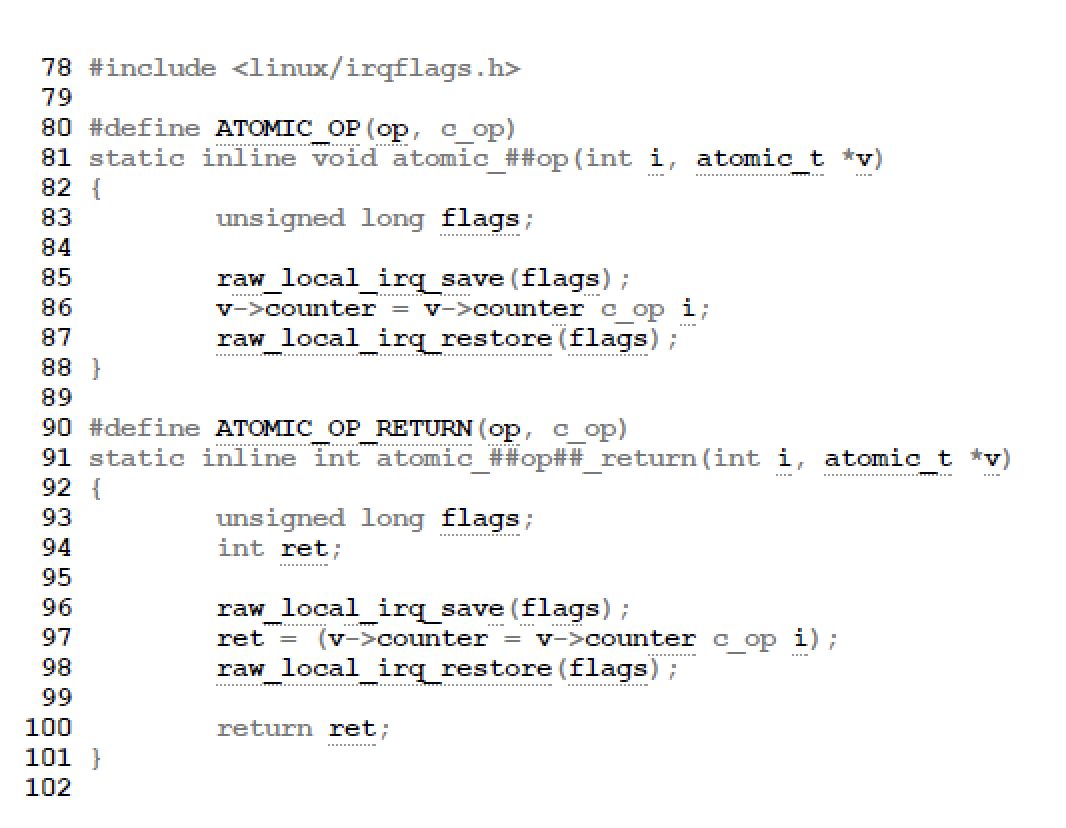
\includegraphics[scale=0.45]{Linux_generic_atomic.png}
  \caption{Generic Atomic Operations in Linux/include/asm-generic/atomic.h}
  \label{fig:ec}
\end{figure}\\
However, the approach we mentioned above does not utilize the atomic operations supported by the hardware. Thus, it is generally slower. For different architectures, Linux provides different implementation of atomic operations. Our discussion will focus on two most common architectures: x86 and ARM.\\

\subsection{Atomic Operations on ARM Architecture}
On Arm architecture, there are existing atomic instructions. Thus, Linux utilized them to perform atomic operations directly. On architectures with ARMv5 or earlier version, Linux utilizes swp operations to implement atomic operations.\\
swp Rd Rm Rn\\
- Rn contains an address space in memory.\\
- Data from memory is loaded into Rd .\\
- Content of Rm is saved in memory.\\
- If Rd == Rm, swap content of register and memory.\\
There is a special case, on StrongARM CPU, the implementation of swp operation is itself bogus, since it totally bypasses the cache. Linux developer decided to use the basic method to solve this problem: disable interrupts, emulate atomic operations, re-enable interrupts.\\
On architecture with ARMv6 or later version, Linux relies on LDREX and STREX instructions to implement atomic operations.\\
LDREX Rd, [Rn]\\
- RD is the destination register. After completion, it contains the data loaded from memory.\\
- Rn is the register holding the memory.\\
LDREX instruction guarantees that the current processor has the exclusive access to the physical address loaded.\\
STREX Rd, Rm, [Rn]\\
- RD is the destination register. After completion, it contains either 0 (if the instruction succeed), or 1 (if the instruction is locked out).
- Rm is the source register holding the data to store to memory.
- Rn is the register holding the memory address.\\
STREX performs an atomic store to the memory.\\
The detailed usages of those instructions we mentioned above in Linux kernel is in Linux/arch/arm/include/asm/atomic.h. The code utilizing LDREX andd STREX is posted below.\\

\begin{figure}[h!]
  \centering
  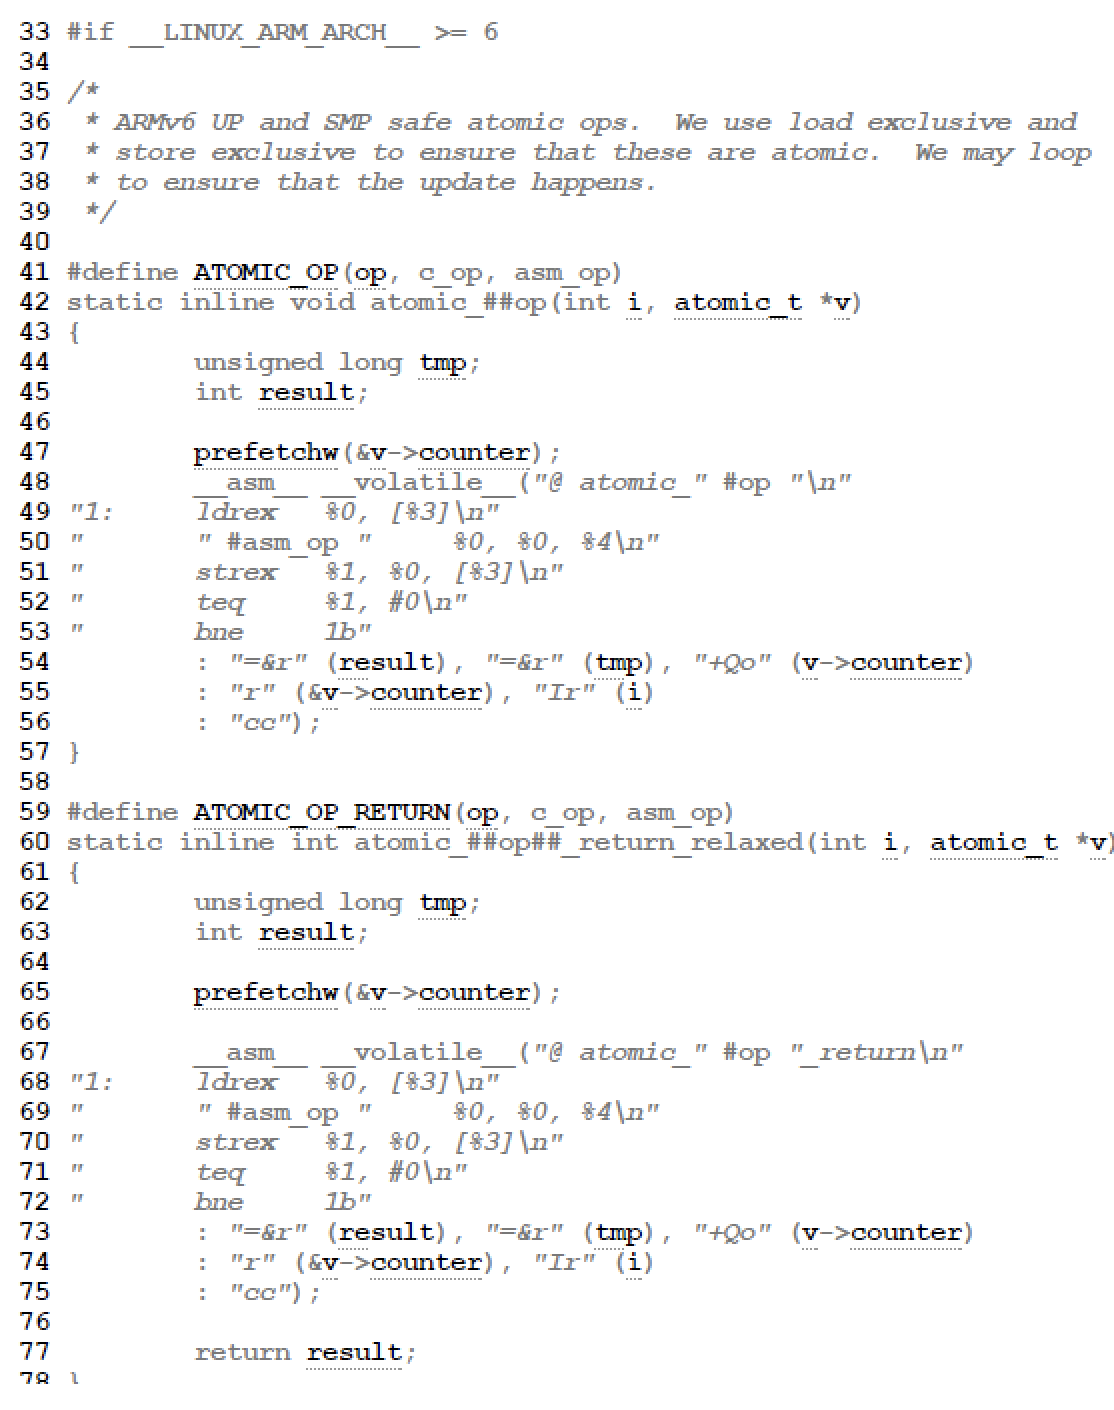
\includegraphics[scale=0.45]{ARM_atomic.png}
  \caption{Atomic Operations for ARM Architecture in Linux/arch/arm/include/asm/atomic.h}
  \label{fig:ec}
\end{figure}

\vspace{100pt}

\subsection{Atomic Operations on x86 Architecture}
In x86 architecture, Linux utilizes CMPXCHG instruction to implement atomic operations.\\ 
CMPXCHG Op1 Op2\\
- Op1 is the destination operand. The value in this operand is compared with the AL, AX, or EAX register (depending on the size of the operand). If they are equal, the value in the source operand is loaded into the destination operand. Otherwise, the value in the destination operand is loaded into the AL, AX, or EAX register.\\
- Op2 is the source operand.\\
When CMPXCHG instruction is used with LOCK prefix, the instruction is done atomically. Linux utilizes this specific instruction in implementing atomic operations on x86 architecture.\\
The detailed usage of CMPXCHG instructions is in Linux/arch/x86/include/asm/atomic.h. The source code is posted below. Please note that the code posted is in \\Linux/arch/x86/include/asm/cmpxchg.h instead of atomic.h. The reason is that atomic.h utilize cmpxchg.h to implement atomic operations.\\

\begin{figure}[h!]
  \centering
  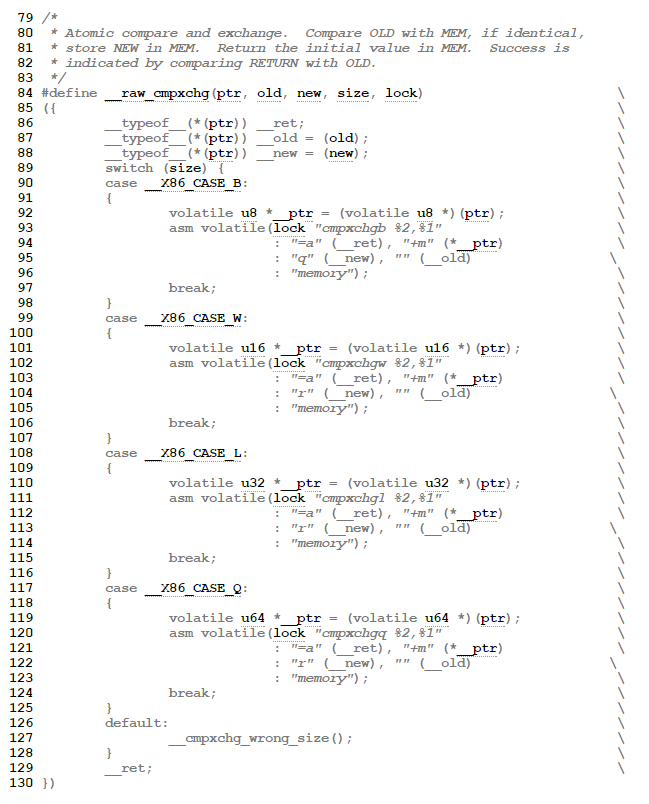
\includegraphics[scale=0.5]{x86_atomic.png}
  \caption{Atomic Operations for x86 Architecture in Linux/arch/x86/include/asm/cmpxchg.h.h}
  \label{fig:ec}
\end{figure}

\subsection{Summary}
Atomic operation itself is a good example of the functionality of an operating system. From a user's perspective, atomic operations are always supported, while the implementation details are hidden. From hardware's perspective, an atomic operation is simply a sequence of instructions. Operating system successfully decouples the user interface and hardware implementation details. Moreover, atomic operation is also a good example of the cooperation between software and hardware. With support from hardware, atomic operation can be implemented efficiently. \\

\vspace{50pt}

\section{Approaches and Tools}
The analysis of Linux source code is done on the website of Linux Cross Reference (http://lxr.free-electrons.com/source/). We analyzed on the latest version (4.10) and did not analyze on older version of Linux because our focus in this project is not the development history of mutex subsystem but the actual implementation and design highlights of mutex subsystem.\\
\subsection{For Implementation and Design Highlights of Linux Mutex Subsystem}
We first read the design doc of Linux Mutex Subsystem (Linux/Documentation/mutex-design.txt). After understanding the design of mutex subsystem, we looked thoroughly into the source code for mutex to figure out how the design is implemented in Linux kernel source code. \\
After all those steps, we have had a good understanding of the implementation of mutex subsystem and found ourselves very interested in the unique optimistic spinning phase of mutex locking routine. Therefore, we started to look into the optimistic spinning phase and the special MCS locks used in optimistic spinning. \\

\subsection{For Linux Implementation of Atomic Operations}
Besides from linux source code, we relied on\\ http://infocenter.arm.com/help/index.jsp to check the ARM instructions and http://x86.renejeschke.de to check x86 instructions. \\

\vspace{50pt}

\section{Conclusion}
It's obvious that we should prefer to use mutex over semaphore in the future while we are developing multi-thread programs because of the various advantages of struct mutex. \\
In addition, we found ourselves inspired by the optimistic spinning phase of Linux mutex locking routine because the same idea of a few cycles of busy waiting before putting a thread to sleep can be used in many other concurrency control scenarios. For example, in our own multi-thread programs if we are entering a particular critical section but fails to acquire the lock at the current point, we can have a busy loop to try to acquire the lock several times before we block the current thread by the actual .lock() function call. 

\vspace{50pt}


\section{Reference}
http://lxr.free-electrons.com/source/Documentation/mutex-design.txt?v=3.10\\

\noindent http://lxr.free-electrons.com/source/kernel/locking/mcs\_spinlock.h\\

\noindent https://lwn.net/Articles/590243/\\

\noindent https://lwn.net/Articles/575460/\\

\noindent https://lwn.net/Articles/600111/\\

\noindent http://infocenter.arm.com/help/index.jsp\\

\noindent http://x86.renejeschke.de



\end{document}

\bibliographystyle{acm}
% \bibliography{xxx}

\end{document}
